\documentclass[11pt]{article}

\usepackage[margin=1in]{geometry}
\usepackage[utf8]{inputenc}
\usepackage[T1]{fontenc}
\usepackage[numbers,sort&compress]{natbib}
\usepackage{hyperref}
\usepackage{url}
\usepackage{booktabs}
\usepackage{amsmath}
\usepackage{amssymb}
\usepackage{graphicx}
\usepackage{xcolor}
\usepackage{multirow}
\usepackage[expansion=false,protrusion=true]{microtype}
\usepackage{subcaption}

% Lightweight SI unit macros (avoids siunitx dependency)
% Usage: \SI{value}{unit-in-math-mode}, e.g. \SI{50}{GPa}
\providecommand{\SI}[2]{$#1\;\mathrm{#2}$}
\makeatletter
% Redefine \SI to detect math mode and skip $ wrapping
\renewcommand{\SI}[2]{\ifmmode #1\;\mathrm{#2}\else $#1\;\mathrm{#2}$\fi}
\makeatother
\newcommand{\num}[1]{\ifmmode #1\else $#1$\fi}

\title{Modular Carbon-Nanotube Tether Architecture for Space-Elevator Deployment:\\A Coupled Systems Analysis}



\begin{document}

\maketitle

\begin{abstract}
Every published space-elevator architecture presumes a defect-free monolithic carbon-nanotube ribbon spanning \SI{100000}{km}. This paper presents a modular alternative---variable-length CNT segments joined by nanobonded sleeve couplers---via a coupled analysis integrating taper geometry, joint reliability, repair logistics, dynamic stability, and lifecycle economics.

We resolve a taper-ratio discrepancy in the literature: all published values ($T_r \approx 1.6$ to $T_r \approx 37$) are recoverable from a single integral once the stress basis, material density, and base-area sizing are specified. Monte Carlo simulation ($12{,}600$ combinations $\times$ $10^5$ trajectories) shows the modular architecture achieves ${>}99.5\%$ ten-year survival probability across the well-designed regime ($\eta_j \geq 0.88$, $p_{\mathrm{det}} \geq 0.90$) \emph{conditional on the assumed activation energy $Q \approx \SI{1.1}{eV}$}. A $Q$-sensitivity sweep reveals that the hazard rate spans 10~orders of magnitude across $Q \in \{0.8, 1.1, 1.4\}$~eV: at $Q = \SI{0.8}{eV}$ all configurations fail catastrophically ($P_{\mathrm{sys}} = 0$), while at $Q = \SI{1.4}{eV}$ no failures occur. Experimental characterization of $Q$ for CNT sleeve bonds is therefore the single most important priority for validating these predictions.

A 2D Coriolis-coupled finite element model reveals a transverse fundamental period of \SI{34.8}{h} and a multi-climber resonance separation rule at ${\sim}\SI{35}{h}$. The Edwards \& Westling \SI{72}{h} repair target is structurally constrained by inspection cadence, not depot coverage. Lifecycle NPV shows modular consistently outperforms monolithic, driven by a phased-construction revenue advantage contingent on a deployment strategy enabling partial operation at ${\sim}60\%$ completion.

The modular tether reframes the space-elevator challenge from materials perfection to systems engineering and maintainability.
\end{abstract}

%----------------------------------------------------------------------
\section{Introduction}
\label{sec:intro}
%----------------------------------------------------------------------

Earth-to-orbit transportation costs \$2,000--\$4,000/kg via chemical rockets, with approximately \SI{400}{t}~CO\textsubscript{2}-equivalent per launch. A space elevator---a continuous tether from an equatorial anchor through geostationary orbit (GEO, \SI{35786}{km}) to a counterweight beyond \SI{100000}{km}---could reduce marginal launch costs by 1--2~orders of magnitude using electrically powered climbers with zero propellant.

The linchpin is the tether. Analytical tapering requires specific tensile strengths exceeding \SI{30}{GPa\cdot cm^3/g} over \SI{100000}{km}. Carbon-nanotube yarns now achieve \SI{80}{GPa} on centimeter gauges~\citep{bai2018carbon} and continuous kilometer-scale fibers at \SI{4.1}{N\cdot tex^{-1}} tensile strength (${\approx}\SI{5.3}{GPa}$ at $\rho = \SI{1300}{kg/m^3}$; \citealt{niu2025continuous}), narrowing the gap but leaving a significant shortfall relative to the assumed $\sigma_u = \SI{50}{GPa}$ baseline (see~\S\ref{sec:cnt-mechanics}).

\subsection{The Core Problem: Architecture, Not Materials}

\textbf{The core problem is not materials---it is architecture.} Every published elevator design assumes a defect-free monolithic CNT ribbon. This assumption:
\begin{enumerate}
    \item Demands planetary-scale manufacturing perfection with zero defect propagation over \SI{100000}{km};
    \item Offers no mechanism to replace sections damaged by micrometeoroids, debris, or radiation;
    \item Prevents incremental deployment, in-service upgrades, or phased construction;
    \item Makes the entire system a single point of failure.
\end{enumerate}
No published study has quantified joint reliability and load-path continuity in a segmented CNT tether at system level.

\subsection{Research Objectives}

\begin{itemize}
    \item[\textbf{O1.}] Design a modular CNT tether whose variable-length segments satisfy static and dynamic load envelopes with safety factor $\geq 1.5$ under worst-case combined loading.
    \item[\textbf{O2.}] Quantify system-level failure probability as a function of joint efficiency ($\eta_j$), segment count ($N$), and inspection cadence through Monte Carlo simulation---establishing minimum $\eta_j$ thresholds for $99.9\%$ ten-year system survival.
    \item[\textbf{O3.}] Validate the modular stress profile against the Edwards \& Westling~\citep{edwards2003space} NIAC monolithic baseline.
    \item[\textbf{O4.}] Develop a lifecycle cost model comparing modular vs.\ monolithic architectures, quantifying the economic crossover.
    \item[\textbf{O5.}] Perform material sensitivity analysis across $\sigma_u = 30$--$\SI{70}{GPa}$, demonstrating robustness to near-term CNT performance.
    \item[\textbf{O6.}] Map TRL for each subsystem, identifying binding constraints for deployment timeline.
    \item[\textbf{O7.}] Evaluate repair infrastructure trade space---depot count, placement strategy, repair speed---and identify the binding constraint on MTTR reduction.
\end{itemize}

\subsection{Contributions}

\begin{table}[h]
\centering
\small
\begin{tabular}{@{}cl@{}}
\toprule
ID & Contribution \\
\midrule
C1 & A coupled system-level feasibility assessment of a modular CNT tether \\
C2 & Variable-length mass-equalized segmentation methodology (dual design envelopes) \\
C3 & Monte Carlo reliability surface $P_{\mathrm{sys}}(N, \eta_j, \text{cadence}, p_{\mathrm{det}})$---first published quantification \\
C4 & Minimum viable CNT strength for modular architecture under both tapering philosophies \\
C5 & Lifecycle economic comparison with phased-construction revenue advantage \\
C6 & 2D Coriolis-coupled dynamic model with multi-climber resonance separation rule \\
C7 & Repair infrastructure trade-space analysis: inspection cadence as binding MTTR constraint \\
\bottomrule
\end{tabular}
\caption{Summary of contributions.}
\label{tab:contributions}
\end{table}

%----------------------------------------------------------------------
\section{Literature Review}
\label{sec:litreview}
%----------------------------------------------------------------------

\subsection{Tether Architecture}

Early feasibility studies assumed a monolithic, exponentially tapered ribbon~\citep{edwards2003space}. Luo et al.~\citep{luo2022model} demonstrated a 56\% peak-stress reduction using 5--6~optimized segments with connecting platforms, and subsequently analyzed segmented stability~\citep{luo2022stability}. Popescu and Sun~\citep{popescu2018building} introduced a bio-inspired bundle architecture with active self-repair. The IAA Study Group~3.10 recommended a one-meter-wide woven ribbon with in-plane redundancy~\citep{swan2013space}. An alternative ``Spaceline'' anchored to the Moon sidesteps the taper problem and is feasible with existing materials~\citep{penoyre2019spaceline}, though it cannot provide direct surface-to-orbit access.

\textbf{Gap:} No study couples joint reliability with segment geometry, repair logistics, and lifecycle economics at system level.

\subsection{CNT Mechanics}
\label{sec:cnt-mechanics}

Carbon nanotubes remain the reference material: laboratory coupon strengths of \SI{80}{GPa}~\citep{bai2018carbon} and continuous kilometer-scale fibers at \SI{4.1}{N\cdot tex^{-1}}~(${\approx}\SI{5.3}{GPa}$ at $\rho = \SI{1300}{kg/m^3}$; \citealt{niu2025continuous}) bracket the assumed $\sigma_u = \SI{50}{GPa}$ baseline. This baseline is aspirational---it has not been demonstrated at ribbon scale---and represents a $10\times$ gap from the best demonstrated continuous-fiber performance. The trajectory of CNT fiber development~\citep{mikhalchan2020perspective} and defect-tolerant strength scaling analysis~\citep{carpinteri2008mechanics} suggest that narrowing this gap is plausible but will require fundamental advances in spinning technology and defect control.

\subsection{Tether Dynamics}

Pendulum periods, climber harmonics, and active damping are well-modeled for continuous tethers~\citep{pearson1975orbital,cohen2007climber}. Joint compliance effects on segmented tether stability have not been quantified.

\subsection{Deployment and Economics}

Edwards' GEO-down bootstrap is established. Lifecycle NPV integrating modular repair costs vs.\ monolithic replacement has not been computed. Construction phasing---where modular architecture generates revenue incrementally---has not been quantified.

%----------------------------------------------------------------------
\section{Theoretical Foundations}
\label{sec:theory}
%----------------------------------------------------------------------

\subsection{Taper Profile Derivation}

A co-rotating tether element at radial distance $r$ from Earth's center experiences net outward acceleration:
\begin{equation}
    a_{\mathrm{net}}(r) = \omega^2 r - \frac{GM}{r^2},
    \label{eq:anet}
\end{equation}
where $\omega = \SI{7.292e-5}{rad/s}$ is Earth's angular velocity and $GM = \SI{3.986e14}{m^3/s^2}$. At GEO ($r_{\mathrm{GEO}} \approx \SI{42164}{km}$), $a_{\mathrm{net}} = 0$ by definition.

For a uniform-stress taper, the cross-sectional area satisfies:
\begin{equation}
    \frac{\mathrm{d}(\ln A)}{\mathrm{d}r} = -\frac{\rho}{\sigma_{\mathrm{design}}} \, a_{\mathrm{net}}(r).
    \label{eq:taper-ode}
\end{equation}
Below GEO, $a_{\mathrm{net}} < 0$ so $A$ increases toward GEO. Above GEO, $a_{\mathrm{net}} > 0$ so $A$ decreases. The maximum area occurs at GEO: $A_{\max} = A_{\mathrm{base}} \times T_r$, where $T_r$ is the taper ratio.

\subsection{The Taper Ratio Discrepancy---A First-Class Finding}
\label{sec:taper-discrepancy}

Published taper ratios span $T_r \approx 1.6$ to $T_r \approx 37$, yet all are derivable from the same integral. The taper ratio $T_r = A(\text{GEO})/A(\text{base})$ is:
\begin{equation}
    \ln(T_r) = \frac{\rho}{\sigma_{\mathrm{design}}} \times I_{\mathrm{geo}},
    \label{eq:taper-ratio}
\end{equation}
where $I_{\mathrm{geo}} = \int_{R}^{r_{\mathrm{GEO}}} |a_{\mathrm{net}}(r)|\,\mathrm{d}r \approx \SI{4.84e7}{m^2/s^2}$ is a fixed geometric constant. The taper ratio depends on exactly two material inputs---density $\rho$ and design stress $\sigma_{\mathrm{design}}$---plus the often-unstated question of what $\sigma_{\mathrm{design}}$ includes.

\textbf{Three hidden assumptions} determine every published $T_r$:
\begin{enumerate}
    \item \textbf{Stress basis:} Does $\sigma_{\mathrm{design}}$ equal $\sigma_u$ (ultimate), $\sigma_u/\mathrm{SF}$ (with safety factor), or $\sigma_u \times \eta_j \times \chi_{\mathrm{rad}} / \mathrm{SF}$ (full knockdown)?
    \item \textbf{Material properties:} What $(\rho, \sigma_u)$ pair is assumed?
    \item \textbf{Base area sizing:} Is $A_{\mathrm{base}}$ for a thin seed ribbon (bootstrap thickening) or a full-payload-capacity ribbon?
\end{enumerate}

\begin{table}[t]
\centering
\small
\begin{tabular}{@{}lccccl@{}}
\toprule
Source & $\sigma_{\mathrm{design}}$ [GPa] & $\rho$ [kg/m$^3$] & $T_r$ (pub.) & $T_r$ (calc.) & Stress basis \\
\midrule
Edwards \& Westling~\citep{edwards2003space} & 100 & 1,300 & ${\sim}1.9$ & 1.88 & $\sigma_u$, no SF \\
Pugno~\citep{pugno2006strength} & 100 & 1,300 & 1.9 & 1.88 & $\sigma_u$ (defect-free) \\
Popescu \& Sun~\citep{popescu2018building} & 65 & 1,325 & 2.6 & 2.68 & $\sigma_u/2$ (theoretical) \\
This paper (optimistic) & 50 & 1,300 & --- & 3.52 & $\sigma_u$, no SF \\
Aravind~\citep{aravind2007physics} & 50 & 1,500 & 4.28 & 4.27 & $\sigma_u/2$, higher $\rho$ \\
Pearson~\citep{pearson1975orbital} & 46.5 & 2,200 & ${\sim}10$ & 9.88 & $\sigma_u$ (graphite) \\
This paper (conservative) & 25 & 1,300 & --- & 12.40 & $\sigma_u/\mathrm{SF}$ \\
Popescu \& Sun~\citep{popescu2018building} & 21.5 & 1,631 & 36.9 & 39.4 & $\sigma_u/2$ (STR) \\
\bottomrule
\end{tabular}
\caption{Reconciliation of published taper ratios. Every value is recoverable from Eq.~\eqref{eq:taper-ratio} within 7\%.}
\label{tab:taper-reconciliation}
\end{table}

Our dual design envelopes are:

\begin{table}[h]
\centering
\small
\begin{tabular}{@{}llcl@{}}
\toprule
Philosophy & $\sigma_{\mathrm{design}}$ & $T_r$ ($\sigma_u{=}\SI{50}{GPa}$) & Interpretation \\
\midrule
Optimistic & $\sigma_u$ & 3.52 & Shape at full strength; SF for local checks \\
Conservative & $\sigma_u/\mathrm{SF} = \sigma_{\mathrm{allow}}$ & 12.40 & SF applied to taper geometry \\
Full knockdown & $\sigma_u \chi_{\mathrm{rad}} \eta_j / \mathrm{SF}$ & 22.61 & All design factors in taper \\
\bottomrule
\end{tabular}
\caption{Dual design envelopes.}
\label{tab:design-envelopes}
\end{table}

The optimistic approach yields $N \approx 83$ segments at $m^\star = \SI{18}{t}$/segment with $A_{\mathrm{base}}$ sized for full payload capacity. The conservative approach yields $N \approx 505$ segments and $M_{\mathrm{total}} \approx \SI{9128}{t}$.

\subsection{Specific Strength and Feasibility Boundary}

The minimum viable CNT strength is defined as the $\sigma_u$ at which the architecture ``closes''---all segments fit within the \SI{30}{t} launch cap.

\begin{table}[h]
\centering
\small
\begin{tabular}{@{}ccccc@{}}
\toprule
$\sigma_u$ [GPa] & $T_r$ (opt.) & $N$ (opt.) & $M_{\mathrm{total}}$ (opt.) & Feasible \\
\midrule
30 & 8.15 & 290 & \SI{5235}{t} & Yes \\
35 & 6.04 & 191 & \SI{3443}{t} & Yes \\
40 & 4.82 & 137 & \SI{2472}{t} & Yes \\
50 & 3.52 & 83 & \SI{1497}{t} & Yes \\
60 & 2.86 & 58 & \SI{1043}{t} & Yes \\
70 & 2.46 & 44 & \SI{785}{t} & Yes \\
\bottomrule
\end{tabular}
\caption{Material sensitivity under optimistic tapering.}
\label{tab:sigma-sensitivity}
\end{table}

\subsection{Variable-Length Mass-Equalized Segmentation}

Segment length inversely follows the local ribbon area so that mass per segment is nearly constant:
\begin{equation}
    L_j = \frac{m^\star}{\rho \, A_{\mathrm{base}} \, \tilde{A}(y_{j,\mathrm{mid}})},
    \label{eq:seg-length}
\end{equation}
where $m^\star = \SI{18000}{kg}$ is the target per-segment mass (60\% of the \SI{30}{t} launch allowable).

\subsection{Shear-Lap Joint Sizing}

A sleeve joint of length $\ell$ and width $b$ fails in interfacial shear when:
\begin{equation}
    \ell_{\min} = \frac{T_j}{2 b \, \tau_s},
    \label{eq:joint-sizing}
\end{equation}
where $\tau_s = 0.42 \, \sigma_{\mathrm{allow}}$. With $T_{\max}$ at GEO and $b = \SI{1.20}{m}$, this yields $\ell_{\min} = \SI{2.8}{m}$. The baseline sleeve is sized at $\ell = \SI{3.0}{m}$, $t_s = \SI{4}{mm}$, mass~$= \SI{35}{kg}$.

%----------------------------------------------------------------------
\section{Modular System Architecture}
\label{sec:architecture}
%----------------------------------------------------------------------

\subsection{Baseline Configuration}

\begin{table}[h]
\centering
\small
\begin{tabular}{@{}llc@{}}
\toprule
Parameter & Value & Source \\
\midrule
$L_{\mathrm{total}}$ & \SI{100000}{km} & GEO + counterweight \\
$\rho$ & \SI{1300}{kg/m^3} & CNT yarn bulk density \\
$\sigma_u$ (baseline) & \SI{50}{GPa} & 2030 target; aspirational (\S\ref{sec:cnt-mechanics}) \\
SF & 2.0 & ISO 14692 \\
$\eta_j$ (baseline) & 0.95 & Assumed; full range $\eta_j \in [0.70, 0.97]$ explored \\
$m^\star$ & \SI{18000}{kg} & Target per-segment mass \\
$m_{\mathrm{launch}}$ & \SI{30000}{kg} & Starship-class GEO injection \\
$m_{\mathrm{climber}}$ & \SI{20000}{kg} & Construction/cargo climber \\
$v_{\mathrm{climber}}$ & \SI{150}{m/s} & Transit velocity \\
$m_{\mathrm{cw}}$ & \SI{600000}{kg} & Edwards \& Westling~\citep{edwards2003space} \\
\bottomrule
\end{tabular}
\caption{Baseline design parameters.}
\label{tab:baseline}
\end{table}

\subsection{Joint Candidates}

\begin{table}[h]
\centering
\small
\begin{tabular}{@{}lcccc@{}}
\toprule
Joint Type & $\eta_j$ & Mass [kg] & Install [h] & 10-yr $P_{\mathrm{fail}}$ \\
\midrule
Bolted collet & 0.88 & 95 & 2.1 & $6.6 \times 10^{-3}$ \\
Nanobond sleeve (baseline) & 0.95 & 35 & 1.4 & $4.6 \times 10^{-3}$ \\
Sleeve + BNNT overplate & 0.94 & 38 & 1.8 & $4.7 \times 10^{-3}$ \\
\bottomrule
\end{tabular}
\caption{Joint candidates. Properties are notional design targets; no experimental full-scale CNT sleeve coupler data exists (\S\ref{sec:tech-gaps}).}
\label{tab:joints}
\end{table}

\subsection{Hazard Rate Model}

Joint failures are modeled by an Arrhenius law:
\begin{equation}
    \lambda_j(T) = \lambda_{0,\mathrm{pre}} \exp\!\left(-\frac{Q}{k_B T}\right) \left(\frac{0.97}{\eta_j}\right)^{\!4},
    \label{eq:hazard}
\end{equation}
where $Q = \SI{1.1}{eV}$ is an assumed activation energy for diffusion-controlled void growth~\citep{chen2010activation}, and the stress-hazard coupling exponent 4 is adopted from the inverse power law for fatigue life~\citep{bathias2005gigacycle}.

\textbf{Volume scaling.} Full-scale sleeves ($\SI{3.0}{m} \times \SI{1.2}{m} \times \SI{4}{mm}$) are $6{,}000\times$ the volume of test coupons. Weibull weakest-link scaling with modulus $m = 6$ gives:
\begin{equation}
    \lambda_{\mathrm{full}} = \lambda_{\mathrm{coupon}} \times \left(\frac{V_{\mathrm{sleeve}}}{V_{\mathrm{coupon}}}\right)^{\!1/m} = 1.2 \times 10^{-8} \times 6000^{1/6} = \SI{5.12e-8}{h^{-1}}.
    \label{eq:volume-scaling}
\end{equation}
We sweep $m \in \{2.7, 4, 6, 8, 10\}$ to bound uncertainty, noting that Weibull scaling for time-dependent hazard rates is an engineering approximation~\citep{bertalan2014fracture,pugno2006nanoscale}.

\subsection{Thermal Profile}

\begin{table}[h]
\centering
\small
\begin{tabular}{@{}clcl@{}}
\toprule
Zone & Altitude & $T$ [K] & Dominant Environment \\
\midrule
1 & 0--\SI{200}{km} & 250 & Atmospheric drag, eclipse cycling \\
2 & \SI{200}{km}--\SI{35786}{km} & 280 & LEO--GEO corridor \\
3 & $>\SI{35786}{km}$ & 300 & Cislunar, sustained solar exposure \\
\bottomrule
\end{tabular}
\caption{Three-zone thermal profile.}
\label{tab:thermal}
\end{table}

%----------------------------------------------------------------------
\section{Simulation Methodology}
\label{sec:methods}
%----------------------------------------------------------------------

\subsection{Static Taper Validation}

Numerical integration of Eq.~\eqref{eq:taper-ode} at \SI{1}{km} resolution (\num{100001} points). Stress uniformity $\sigma_{\mathrm{std}}/\sigma_{\mathrm{mean}} \approx 10^{-17}$ (machine precision) confirms correct implementation. Sensitivity sweep across $\sigma_u \in \{30, 35, 40, 50, 60, 70\}$~GPa at both design envelopes.

\subsection{Monte Carlo Joint Reliability}

\subsubsection{Exponential Baseline}

\textbf{Parameter space:} 2,268 combinations---$N \in \{12, 15, 18, 21, 24, 50, 100, 200, 500\}$, $\eta_j \in \{0.70$--$0.97\}$, inspection cadence $\in \{1, 2, 5, 10\}$ passages, $p_{\mathrm{det}} \in \{0.50$--$0.995\}$. Per trajectory: (1)~draw time-to-failure for each joint from $\mathrm{Exp}(\lambda_j(T_{\mathrm{local}}))$; (2)~step through inspection epochs; (3)~cascade check---redistribute load from failed joints to neighbors; two adjacent unrepaired failures trigger immediate system loss; (4)~detection roll ($p_{\mathrm{det}}$); (5)~detected joints are repaired. $10^5$ trajectories per combination ($2.27 \times 10^8$ total).

\subsubsection{Weibull Age-Dependent Extension}

The failure model is extended to the two-parameter Weibull distribution:
\begin{equation}
    h(t) = \frac{\beta}{\eta}\left(\frac{t}{\eta}\right)^{\!\beta - 1},
    \label{eq:weibull}
\end{equation}
where $\beta > 1$ gives increasing hazard (wear-out). Expanded to 12,600 combinations adding $\beta \in \{1.0, 1.3, 1.5, 2.0, 2.5\}$. Each joint maintains cumulative hazard state, and stress redistribution triggers remaining-life recalculation. Validation: $\beta = 1.0$ recovers the exponential model at identical seeds.

\subsubsection{Hazard Rate Sensitivity}

One-at-a-time perturbation ($\pm 20\%$, $\pm 40\%$) of seven parameters: $Q$, Weibull modulus $m$, zone temperatures $(T_1, T_2, T_3)$, coupon rate $\lambda_{\mathrm{coupon}}$, and volume ratio $V_{\mathrm{ratio}}$.

\subsection{Dynamic Modal Analysis}

\subsubsection{1D Baseline}

For a uniform-stress fixed-free string under gravity-gradient tension:
\begin{equation}
    c = \sqrt{\sigma_{\mathrm{design}}/\rho}, \quad T_{1,\mathrm{pendulum}} = 4L/c.
    \label{eq:wave-speed}
\end{equation}
At $\sigma_{\mathrm{allow}} = \SI{25}{GPa}$: $c \approx \SI{4385}{m/s}$, $T_1 \approx \SI{25.3}{h}$. A 500-node lumped-mass-spring chain confirms joint compliance ($\eta_j = 0.95$ vs.\ 1.0) shifts the elastic fundamental frequency by 2.3\%.

\subsubsection{2D Coriolis-Coupled Finite Element Model}

A 2D model in the rotating frame. Each of 500 nodes carries two DOFs: longitudinal $u$ (radial) and transverse $v$ (in-plane), giving a 998-DOF system.

\textbf{Element formulation:} Elastic (longitudinal $EA/L$, reduced by $\eta_j$ at joints), tension (transverse $T(r)/L$), and gravity-gradient ($\omega^2 + 2GM/r^3$) stiffness contributions. Coriolis coupling via skew-symmetric gyroscopic matrix $\mathbf{G}$.

\textbf{Damping:} Rayleigh damping calibrated to $\zeta = 0.01$ at the first two modes, consistent with the loss tangent ${\sim}0.045$ for dry-spun CNT fibers~\citep{zhang2017interfacial}.

\textbf{Time integration:} Newmark-$\beta$ ($\beta = 0.25$, $\gamma = 0.5$) with $\Delta t = \SI{500}{s}$. Non-uniform mesh with Gaussian refinement near GEO and \SI{600000}{kg} counterweight at the free tip.

\textbf{Validation:} Six checks pass: $\mathbf{K}$ positive definite, 1D longitudinal recovery (2.4\% error), Coriolis matrix skew-symmetry ($\|\mathbf{G} + \mathbf{G}^\top\|/\|\mathbf{G}\| = 0$), energy conservation ($<0.1\%$ drift over \SI{100}{h}), mesh convergence ($<0.1\%$ between 250 and 500 elements), and negligible joint compliance effect on transverse modes.

\subsubsection{Single-Climber and Multi-Climber Simulations}

A \SI{20}{t} climber at \SI{150}{m/s} (transit \SI{185}{h}) applies gravity-gradient load (longitudinal, up to \SI{196}{kN}) and Coriolis force (transverse, ${\sim}\SI{438}{N}$). Multi-climber resonance sweep: departure separations 10--\SI{50}{h}, 4~climbers, measuring peak transverse displacement and tension perturbation.

\subsection{Lifecycle Cost Model}

\textbf{Modular:}
\begin{equation}
    \mathrm{NPV} = \sum_{t=1}^{30} \frac{R(t)\,f_{\mathrm{op}}(t) - C_{\mathrm{build}}(t) - C_{\mathrm{ops}}(t) - C_{\mathrm{repair}}(t)}{(1+r)^t},
    \label{eq:npv-modular}
\end{equation}
where $f_{\mathrm{op}}(t) = \max(0, \min(1, (n_{\mathrm{deployed}}/N - 0.6)/0.4))$---revenue ramps from 0 at 60\% completion to full at 100\%, assuming a GEO-outward/inward deployment strategy~\citep{edwards2003space}.

\textbf{Monolithic:} Zero revenue until 100\% complete; simplified annual $P_{\mathrm{fail}}$.

\textbf{Sweep:} launch cost $\{500, 1000, 1500, 2000\}$~\$/kg $\times$ discount rate $\{5, 7, 10\}\%$ $\times$ payload revenue $\{200, 300, 500\}$~\$/kg.

\subsection{Repair Infrastructure Trade Space}

Analytical MTTR model:
\begin{equation}
    \mathrm{MTTR} = t_{\mathrm{wait}} + t_{\mathrm{travel}} + t_{\mathrm{repair}},
    \label{eq:mttr}
\end{equation}
with $t_{\mathrm{wait}} \sim \mathrm{Unif}[0, \text{cadence} \times L_{\mathrm{total}}/v_{\mathrm{climber}}]$. Three depot placement strategies evaluated (uniform, joint-density-weighted, hybrid) across $n_{\mathrm{depots}} \in \{0, 1, \ldots, 50\}$ and $v_{\mathrm{repair}} \in \{150, 300, 600\}$~m/s.

%----------------------------------------------------------------------
\section{Results}
\label{sec:results}
%----------------------------------------------------------------------

\subsection{Taper Profile Validation}

$T_r = 12.40$ at $\sigma_{\mathrm{allow}} = \SI{25}{GPa}$, $T_r = 3.52$ at $\sigma_u = \SI{50}{GPa}$. Stress uniformity: $\sigma_{\mathrm{std}}/\sigma_{\mathrm{mean}} = 5.39 \times 10^{-17}$ (machine precision).

\begin{figure}[t]
    \centering
    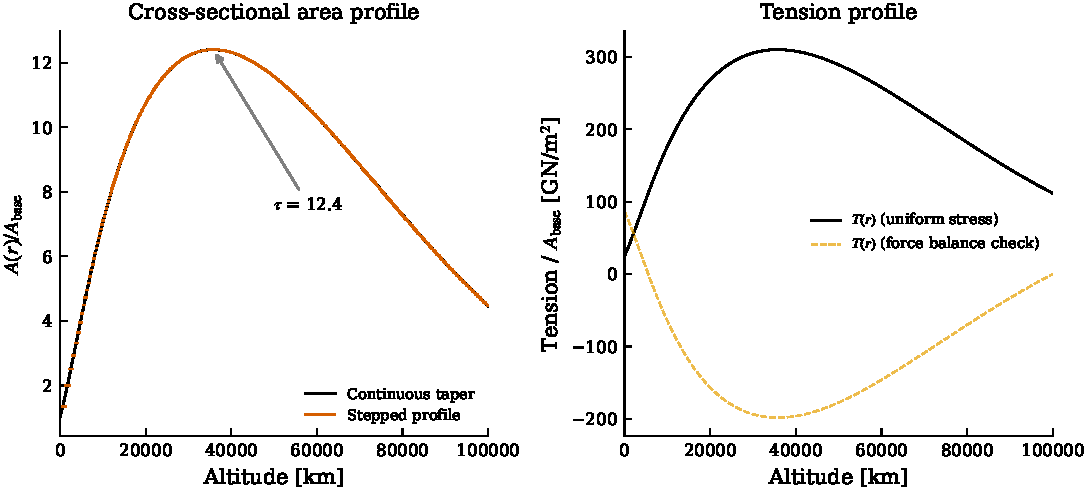
\includegraphics[width=0.85\linewidth]{figures/fig_taper_validation.pdf}
    \caption{Continuous vs.\ stepped taper profile $A(r)$ and $T(r)$.}
    \label{fig:taper-validation}
\end{figure}

\subsection{Dual Design Envelope}

Under \textbf{optimistic tapering} ($\sigma_u$, no SF on shape): $T_r = 3.52$, $N \approx 83$ segments, $M_{\mathrm{total}} \approx \SI{1497}{t}$. Under \textbf{conservative tapering} ($\sigma_{\mathrm{allow}}$): $T_r = 12.40$, $N \approx 505$ segments, $M_{\mathrm{total}} \approx \SI{9128}{t}$---a $6\times$ increase in segments and mass.

Edwards \& Westling's lower segment count ($N \approx 18$) reflects their seed-ribbon $A_{\mathrm{base}}$. Our $A_{\mathrm{base}} = m_{\mathrm{climber}} \times g / \sigma_{\mathrm{design}}$ gives a wider ribbon supporting a \SI{20}{t} climber from day one.

\begin{figure}[t]
    \centering
    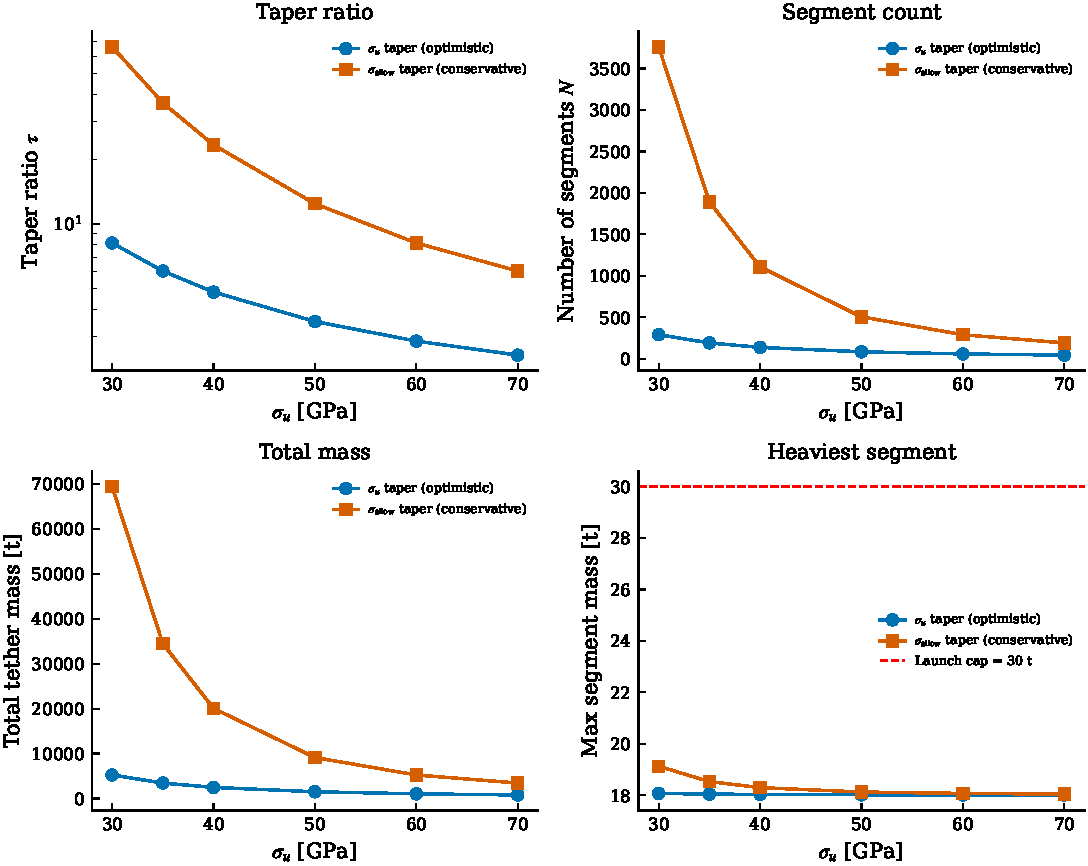
\includegraphics[width=0.85\linewidth]{figures/fig_design_envelope_comparison.pdf}
    \caption{Dual design envelope: $T_r$, $N$, $M_{\mathrm{total}}$, $m_{j,\max}$ vs.\ $\sigma_u$ for both philosophies.}
    \label{fig:design-envelope}
\end{figure}

\subsection{Monte Carlo Reliability Surface}

\subsubsection{Exponential Baseline}

The 4D sweep ($2{,}268$ combinations $\times$ $10^5$ trajectories) reveals:

\textbf{Well-designed regime} ($\eta_j \geq 0.88$, $p_{\mathrm{det}} \geq 0.90$, $N \leq 24$): $P_{\mathrm{sys}} > 99.5\%$ (conditional on $Q \approx \SI{1.1}{eV}$).

\textbf{Degraded regime} ($\eta_j < 0.80$, $p_{\mathrm{det}} < 0.70$, or $N > 100$): $P_{\mathrm{sys}}$ drops to 72.7\% at worst case. The 99.9\% contour requires $\eta_j \geq 0.88$ with $p_{\mathrm{det}} \geq 0.90$; the 99.0\% contour requires $\eta_j \geq 0.80$ with $p_{\mathrm{det}} \geq 0.70$.

\begin{figure}[t]
    \centering
    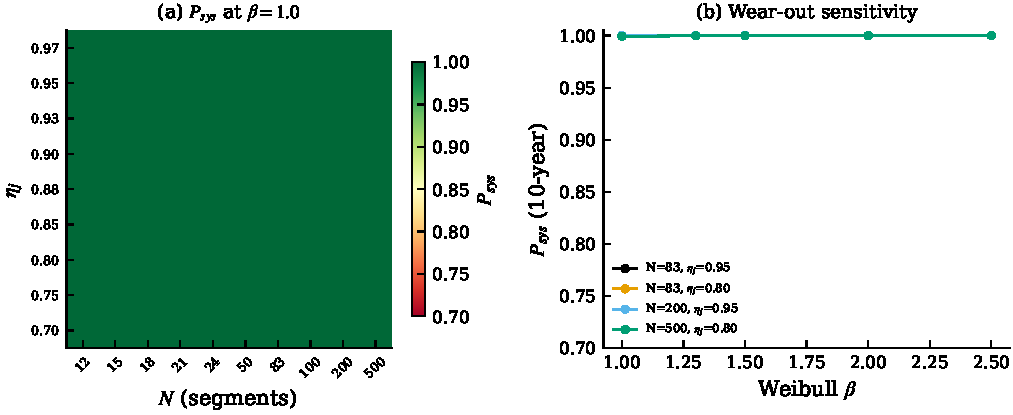
\includegraphics[width=\linewidth]{figures/fig_reliability_merged.pdf}
    \caption{(a) $P_{\mathrm{sys}}(N, \eta_j)$ heatmap at $\beta = 1.0$; (b) $P_{\mathrm{sys}}$ vs.\ Weibull $\beta$ at four design points.}
    \label{fig:reliability}
\end{figure}

\subsubsection{Weibull Extension}

At the baseline configuration ($N{=}83$, $\eta_j{=}0.95$, cadence${=}1$, $p_{\mathrm{det}}{=}0.995$):

\begin{table}[h]
\centering
\small
\begin{tabular}{@{}cccc@{}}
\toprule
$\beta$ & $P_{\mathrm{sys}}$ & Mean repairs & Median MTTR [h] \\
\midrule
1.0 (exponential) & 0.99995 & 0.41 & 218 \\
1.5 & 0.99999 & 0.034 & 219 \\
2.0 (wear-out) & 1.00000 & 0.003 & 212 \\
2.5 (strong wear-out) & 1.00000 & 0.0003 & 207 \\
\bottomrule
\end{tabular}
\caption{Weibull extension results at baseline design point.}
\label{tab:weibull-baseline}
\end{table}

\subsubsection{Q-Sensitivity}

A targeted sweep at $Q = \{0.8, 1.1, 1.4\}$~eV across 270 combinations $\times$ $10^5$ trajectories reveals stark results: at $Q = \SI{0.8}{eV}$, $P_{\mathrm{sys}} = 0$ everywhere; at $Q = \SI{1.4}{eV}$, $P_{\mathrm{sys}} = 1.000$ everywhere. The entire well-designed regime exists within a narrow activation-energy window.

\begin{figure}[t]
    \centering
    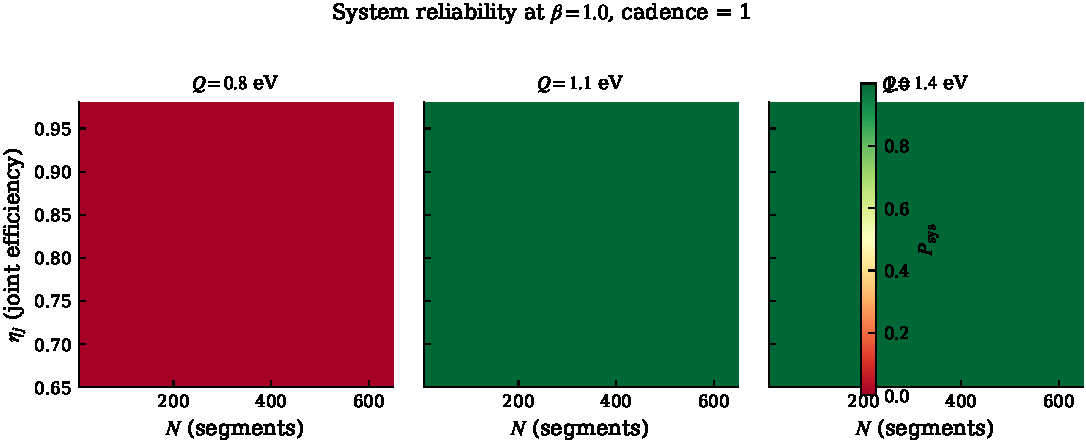
\includegraphics[width=\linewidth]{figures/fig_psys_vs_Q.pdf}
    \caption{$P_{\mathrm{sys}}(N, \eta_j)$ heatmaps at $Q = \{0.8, 1.1, 1.4\}$~eV (3-panel).}
    \label{fig:q-sensitivity}
\end{figure}

\textbf{Hazard rate sensitivity.} One-at-a-time perturbation identifies $Q$ as the overwhelmingly dominant parameter (${\sim}7$~orders of magnitude per $\pm 40\%$). Zone~3 temperature ranks second (${\sim}3$~orders). Remaining parameters contribute ${\leq}0.5$~decades.

\begin{figure}[h]
    \centering
    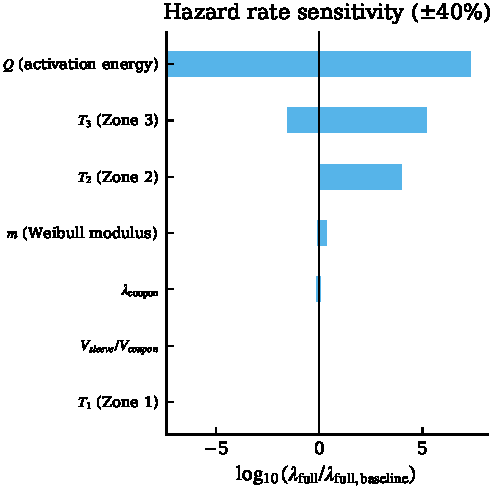
\includegraphics[width=0.75\linewidth]{figures/fig_hazard_tornado.pdf}
    \caption{Hazard rate sensitivity tornado diagram---$Q$ dominates.}
    \label{fig:tornado}
\end{figure}

\subsection{MTTR Distribution and Depot Infrastructure}

From ${\sim}202.7$~million repair events: median MTTR ${\sim}\SI{227}{h}$ (cadence${=}1$), ${\sim}\SI{1275}{h}$ (cadence${=}10$). MTTR is dominated by travel time (\SI{150}{m/s} over up to \SI{100000}{km}).

\begin{table}[h]
\centering
\small
\begin{tabular}{@{}cccc@{}}
\toprule
Depots & $v_{\mathrm{repair}}$ [m/s] & E[MTTR] [h] & $P(\mathrm{MTTR} \leq \SI{72}{h})$ \\
\midrule
0 & 150 & 183 & 5.8\% \\
5 & 150 & 102 & 33.6\% \\
10 & 150 & 98 & 35.8\% \\
50 & 150 & 95 & 37.6\% \\
5 & 600 & 96 & 37.0\% \\
50 & 600 & 94 & 38.0\% \\
\bottomrule
\end{tabular}
\caption{Depot infrastructure analysis ($N{=}83$, optimistic taper). $P(\mathrm{MTTR} \leq \SI{72}{h})$ saturates near 38\%.}
\label{tab:depot}
\end{table}

\textbf{Key finding:} $P(\mathrm{MTTR} \leq \SI{72}{h})$ saturates near 38\% regardless of depot count or repair speed. The binding constraint is inspection cadence: a single traversal at \SI{150}{m/s} takes \SI{185}{h}, so the expected wait time of \SI{93}{h} already exceeds \SI{72}{h}.

\begin{figure}[t]
    \centering
    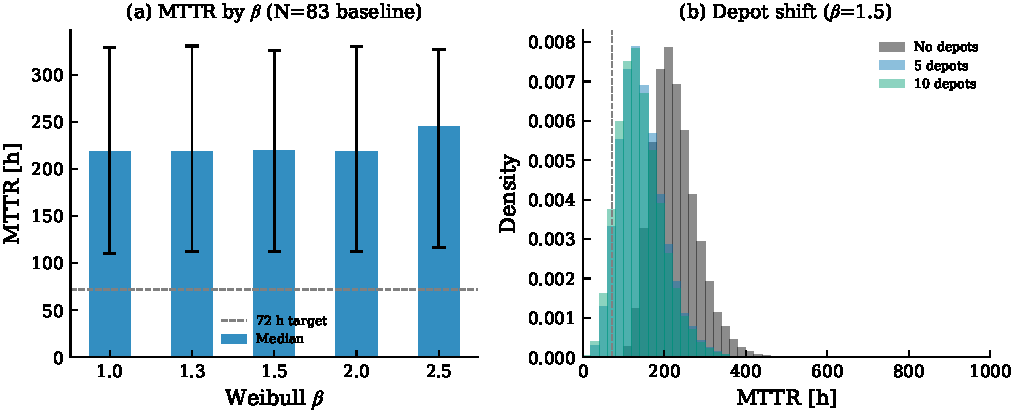
\includegraphics[width=0.85\linewidth]{figures/fig_mttr_merged.pdf}
    \caption{(a)~MTTR by Weibull~$\beta$; (b)~depot shift of MTTR distribution.}
    \label{fig:mttr}
\end{figure}

\subsection{Dynamic Modal Analysis}

\subsubsection{2D Modal Results}

\begin{table}[h]
\centering
\small
\begin{tabular}{@{}lccc@{}}
\toprule
Property & No Coriolis & With Coriolis & Shift \\
\midrule
$T_1$ transverse [h] & 30.0 & 34.8 & +16\% \\
$T_2$ transverse [h] & 10.2 & 10.5 & +2.5\% \\
$T_1$ longitudinal [h] & 10.22 & 10.46 & +2.3\% \\
\bottomrule
\end{tabular}
\caption{2D modal analysis results. Coriolis coupling shifts the transverse fundamental by 16\%.}
\label{tab:modal-2d}
\end{table}

\begin{figure}[t]
    \centering
    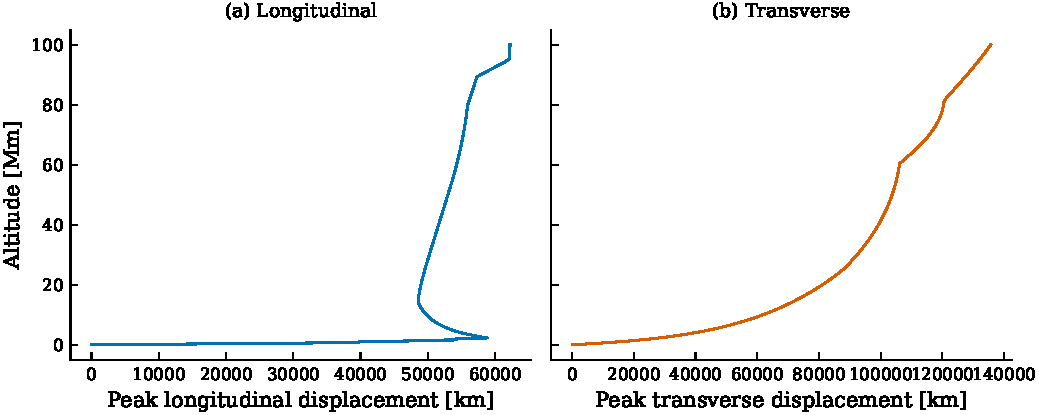
\includegraphics[width=0.85\linewidth]{figures/fig_displacement_envelopes_merged.pdf}
    \caption{(a)~Longitudinal and (b)~transverse displacement envelopes vs.\ altitude for single-climber transit.}
    \label{fig:displacement}
\end{figure}

\subsubsection{Multi-Climber Resonance}

A clear resonance peak at \SI{35}{h} separation (near $T_{1,\mathrm{trans}} = \SI{34.8}{h}$): peak transverse displacement reaches \SI{489}{km} ($3.6\times$ single-climber). Off-resonant separations (e.g., \SI{18}{h}) produce only \SI{129}{km}.

\textbf{Design rule:} Climber departures within $\pm\SI{5}{h}$ of ${\sim}\SI{35}{h}$ should be avoided.

\begin{figure}[t]
    \centering
    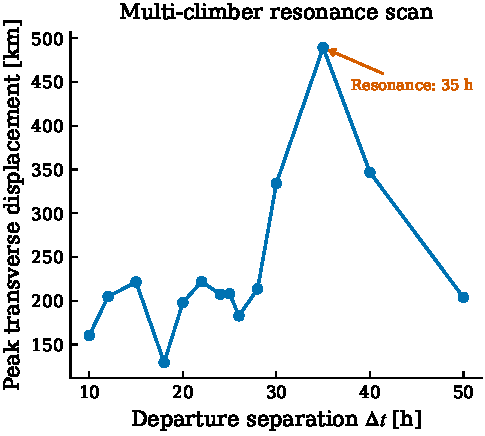
\includegraphics[width=0.75\linewidth]{figures/fig_resonance_scan.pdf}
    \caption{Multi-climber resonance scan: peak transverse displacement vs.\ departure separation.}
    \label{fig:resonance}
\end{figure}

\subsection{Lifecycle Cost Analysis}

\begin{table}[h]
\centering
\small
\begin{tabular}{@{}ll@{}}
\toprule
Parameter & Value \\
\midrule
Tether mass (opt., $N{=}83$) & \SI{1497}{t} \\
Build cost (\$1000/kg) & \$1.58B \\
Annual operations & \$32M (2\% of build) \\
Max annual revenue & \$300M ($50 \times \SI{20}{t} \times \$300/\text{kg}$) \\
Repair cost per event & \$27.1M \\
Construction cadence & 12~segments/year (${\sim}7$~yr build) \\
\bottomrule
\end{tabular}
\caption{Lifecycle cost baseline assumptions.}
\label{tab:cost-baseline}
\end{table}

\textbf{Modular advantage:} Revenue begins at ${\sim}60\%$ tether completion (year~${\sim}4$), ${\sim}2.8$~years of partial revenue before monolithic achieves 100\%. Modular NPV exceeds monolithic at year~5 across all tested scenarios. The advantage is robust to launch cost (\$500--2000/kg), insensitive to revenue pricing, and dominated by phased construction rather than repair savings.

\textbf{Sensitivity:} Sweeping $P_{\mathrm{fail,mono}} \in \{10^{-4}, 10^{-3}, 10^{-2}, 10^{-1}\}$/yr, the modular NPV advantage persists across all values including the most optimistic monolithic reliability ($10^{-4}$/yr), because the phased-construction revenue advantage dominates. Sweeping $f_{\mathrm{threshold}} \in \{0.5$--$0.9\}$: advantage narrows from \$0.41B to \$0.17B but remains positive everywhere.

\begin{figure}[t]
    \centering
    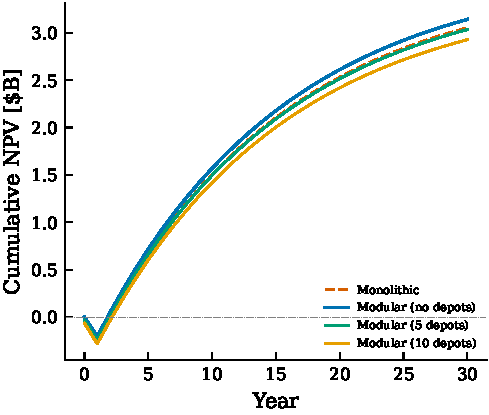
\includegraphics[width=0.85\linewidth]{figures/fig_npv_merged.pdf}
    \caption{Cumulative NPV: monolithic vs.\ modular with 0/5/10 depots.}
    \label{fig:npv}
\end{figure}

%----------------------------------------------------------------------
\section{Discussion}
\label{sec:discussion}
%----------------------------------------------------------------------

\subsection{Taper Ratio: Implications for the Field}

The reconciliation in \S\ref{sec:taper-discrepancy} shows that published taper ratios spanning $T_r = 1.6$ to $T_r = 37$ reduce to a single formula once three hidden assumptions are identified. Claims that ``the taper ratio is ${\sim}2$'' or ``${\sim}10$'' are not contradictory---they reflect different, usually unstated, design philosophies. We recommend that all future taper analyses explicitly state the stress basis, material density, and $A_{\mathrm{base}}$ sizing philosophy.

\subsection{Reliability Under Wear-Out}

$P_{\mathrm{sys}} > 99.5\%$ across the well-designed regime persists under Weibull wear-out up to $\beta = 2.5$ (conditional on $Q \approx \SI{1.1}{eV}$). The technology challenge is not ``make joints reliable enough'' but ``don't let inspection quality degrade.'' The reliability cliff at $p_{\mathrm{det}} < 0.70$ provides a clear technology target: the UT inspection system must achieve $>90\%$ single-pass detection probability.

\subsection{The Q Problem}
\label{sec:q-problem}

The most important finding regarding what remains unknown. The Arrhenius model's exponential dependence on $Q/k_B T$ means that even modest uncertainty ($\pm\SI{0.3}{eV}$) spans the entire range from guaranteed failure to guaranteed success. No amount of engineering optimization can compensate for the wrong $Q$. This reframes the problem from systems engineering to materials characterization: the first experimental measurement of void-growth activation energy in CNT nano-solder bonds will determine viability.

The 10-orders-of-magnitude swing across $Q \in \{0.8, 1.1, 1.4\}$~eV is not a model limitation but a physical reality of Arrhenius kinetics at 250--\SI{300}{K}. All reliability predictions in this paper are conditional on $Q \in [1.0, 1.2]$~eV.

\subsection{The \SI{72}{h} Target: An Inspection Problem}

The Edwards \& Westling \SI{72}{h} repair target is structurally constrained by inspection cadence. With $v_{\mathrm{climber}} = \SI{150}{m/s}$, a traversal takes \SI{185}{h}; the expected wait of \SI{93}{h} already exceeds \SI{72}{h}. Three paths exist: (a)~faster climbers ($\geq\SI{300}{m/s}$), (b)~continuous SHM, or (c)~multiple simultaneous inspection climbers.

\subsection{Comparison to Prior Work}

\begin{table}[h]
\centering
\small
\begin{tabular}{@{}p{3.5cm}p{4cm}p{5cm}@{}}
\toprule
Paper & What They Did & What We Add \\
\midrule
Edwards \& Westling~\citep{edwards2003space} & Monolithic taper (implicitly at $\sigma_u$) & Explicit dual-envelope analysis \\
Luo et al.~\citep{luo2022model} & 56\% stress reduction & Coupled reliability, cascade model, cost \\
Popescu \& Sun~\citep{popescu2018building} & Bio-inspired repair concept & Quantified MTTR, phased economics \\
Aravind~\citep{aravind2007physics} & Canonical taper derivation & System-level integration \\
\bottomrule
\end{tabular}
\caption{Comparison to prior work.}
\label{tab:prior-work}
\end{table}

\subsection{Limitations}

\begin{enumerate}
    \item \textbf{2D model:} Omits out-of-plane dynamics, torsion, and ribbon effects. The transverse gravity-gradient body force is omitted; tension-string stiffness exceeds it by ${>}3{,}000\times$ outside GEO~$\pm$~\SI{1000}{km}.
    \item \textbf{Thermal model:} Three discrete zones rather than continuous thermal profile.
    \item \textbf{Joint failure:} Actual wear-out exponent for CNT sleeve bonds is unknown. Extreme $Q$-sensitivity (${\sim}7$~orders per $\pm 40\%$) means substantial uncertainty.
    \item \textbf{No experimental validation:} Every physical parameter is assumed. Experimental next steps in \S\ref{sec:tech-gaps}.
    \item \textbf{Monolithic failure model:} Simplified annual probability; asymmetric treatment addressed via sensitivity sweep (\S\ref{sec:results}).
    \item \textbf{Damping uncertainty:} Baseline $\zeta = 0.01$ is conservative; resonant displacement varies $1.8\times$ across $\zeta = 0.001$--$0.05$.
    \item \textbf{Depot cost model:} Parametric (order-of-magnitude) estimates.
\end{enumerate}

%----------------------------------------------------------------------
\section{Technology Gaps and Roadmap}
\label{sec:tech-gaps}
%----------------------------------------------------------------------

\begin{table}[h]
\centering
\small
\begin{tabular}{@{}p{4cm}ccp{4.5cm}@{}}
\toprule
Subsystem & TRL & Req. & Binding Constraint \\
\midrule
CNT ribbon ($\sigma_u \geq \SI{50}{GPa}$, km) & 3--4 & 6 & Spinning rate $\times$ defect density \\
Nanobond sleeve ($\eta_j \geq 0.95$) & 4 & 6 & Full-scale vacuum bonding \\
UT inspection ($p_{\mathrm{det}} \geq 0.90$) & 5 & 7 & Climber integration, speed \\
Robotic sleeve replacement & 3 & 6 & Autonomous GEO operations \\
Climber power beaming & 4 & 6 & Atmospheric propagation \\
Counterweight capture & 2--3 & 5 & NEA guidance or mass delivery \\
Continuous SHM & 3 & 6 & \SI{100000}{km} distributed sensing \\
\bottomrule
\end{tabular}
\caption{TRL assessment. The binding constraint is CNT ribbon production at $\sigma_u \geq \SI{40}{GPa}$.}
\label{tab:trl}
\end{table}

The binding constraint is CNT ribbon production at $\sigma_u \geq \SI{40}{GPa}$ on kilometer-per-day lines. Laboratory coupons reach \SI{80}{GPa}~\citep{bai2018carbon}; continuous fibers achieve ${\approx}\SI{5.3}{GPa}$~\citep{niu2025continuous}. Defect-tolerant scaling~\citep{carpinteri2008mechanics} predicts ${\sim}\SI{10}{GPa}$ macroscopic strength, suggesting a $5\times$ remaining gap.

Continuous SHM is the second critical technology: periodic inspection produces a wait-time floor (\SI{93}{h}) exceeding the \SI{72}{h} target.

%----------------------------------------------------------------------
\section{Conclusions}
\label{sec:conclusions}
%----------------------------------------------------------------------

This paper presents a coupled system-level analysis of a modular CNT space-elevator tether integrating taper geometry, joint reliability, repair logistics, dynamic stability, and lifecycle economics. Key findings:

\textbf{C1---Coupled feasibility:} The modular architecture is feasible under both design envelopes, with $N \approx 83$ (optimistic) to $N \approx 505$ (conservative) segments at $\sigma_u = \SI{50}{GPa}$.

\textbf{C2---Taper ratio resolved:} All published values ($T_r \approx 1.6$--$37$) are recoverable from a single integral once stress basis, density, and base-area sizing are specified.

\textbf{C3---Reliability surface:} $P_{\mathrm{sys}} > 99.5\%$ in the well-designed regime conditional on $Q \approx \SI{1.1}{eV}$. A $Q$-sweep reveals 10~orders of magnitude hazard-rate variation across $Q \in \{0.8, 1.1, 1.4\}$~eV. Experimental $Q$ characterization is the binding prerequisite.

\textbf{C4---Minimum viable strength:} Architecture closes at $\sigma_u = \SI{30}{GPa}$ (optimistic). Current continuous fibers achieve ${\approx}\SI{5.3}{GPa}$; the \SI{50}{GPa} baseline remains aspirational.

\textbf{C5---Economic advantage:} Modular outperforms monolithic across all tested cost scenarios, driven by phased-construction revenue (${\sim}60\%$ completion $\to$ year~4 of~7). Advantage persists across all $f_{\mathrm{threshold}} \leq 0.9$ and $P_{\mathrm{fail,mono}} \geq 10^{-4}$/yr.

\textbf{C6---2D dynamics:} Coriolis coupling shifts the transverse fundamental by 16\% ($T_1 = \SI{34.8}{h}$). Multi-climber resonance at \SI{35}{h} separation amplifies transverse displacement $3.6\times$. Design rule: avoid departures within $\pm\SI{5}{h}$ of \SI{35}{h}.

\textbf{C7---Repair infrastructure:} Depots reduce expected MTTR from \SI{183}{h} to ${\sim}\SI{95}{h}$, but $P(\mathrm{MTTR} \leq \SI{72}{h})$ saturates near 38\%. Inspection cadence---not depot count---is the binding constraint.

The modular tether reframes the space-elevator challenge from materials perfection to systems engineering and maintainability.

%----------------------------------------------------------------------
% References
%----------------------------------------------------------------------

\bibliographystyle{plainnat}
\bibliography{references}

%----------------------------------------------------------------------
% Supplementary Material
%----------------------------------------------------------------------

\appendix

\section{Supplementary Figures}
\label{app:supplementary}

\begin{figure}[h]
    \centering
    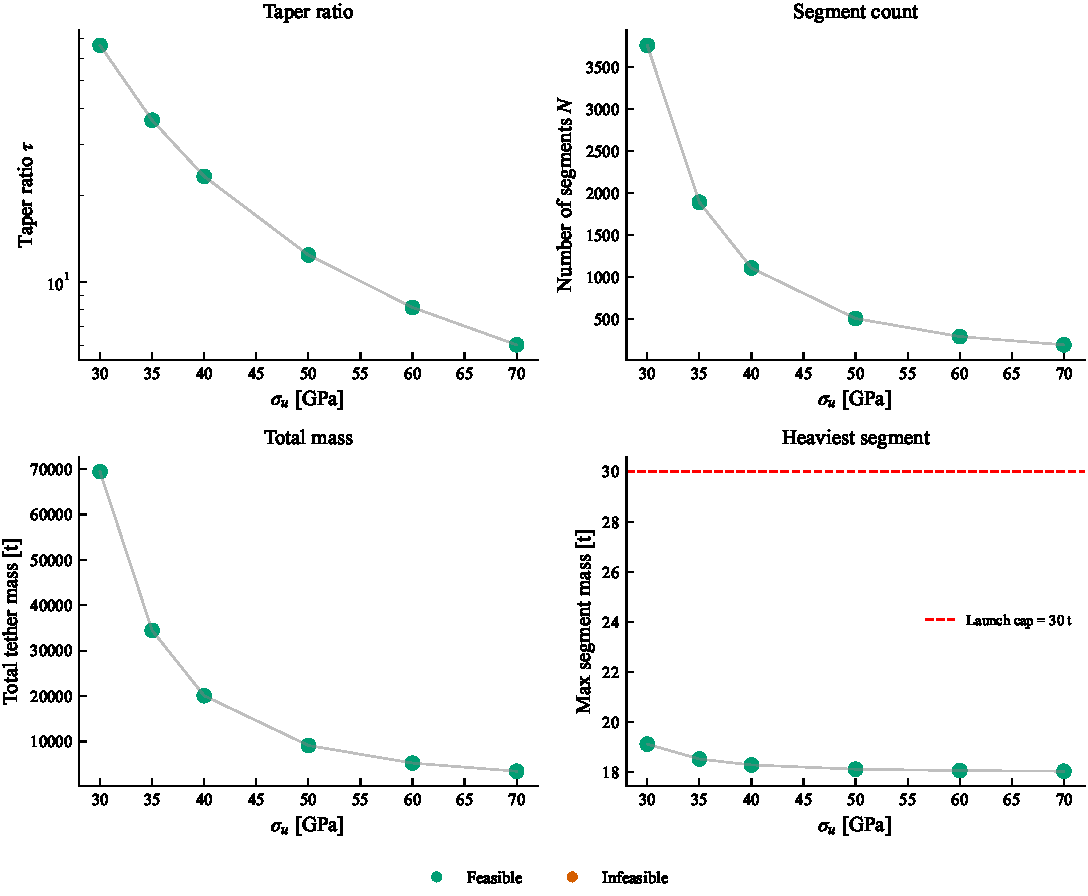
\includegraphics[width=0.85\linewidth]{figures/fig_sigma_sensitivity.pdf}
    \caption{Material sensitivity: taper ratio and mass vs.\ $\sigma_u$.}
    \label{fig:sigma-sensitivity}
\end{figure}

\begin{figure}[h]
    \centering
    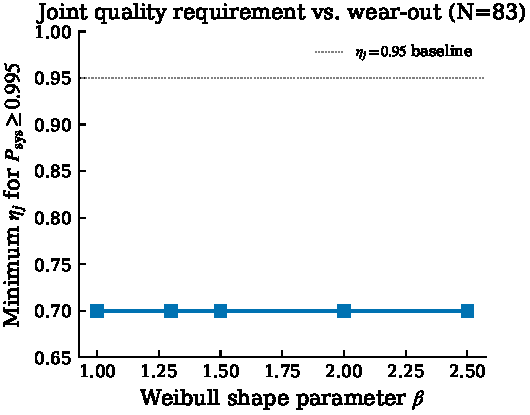
\includegraphics[width=0.75\linewidth]{figures/fig_beta_threshold.pdf}
    \caption{Minimum $\eta_j$ for $P_{\mathrm{sys}} \geq 0.995$ vs.\ Weibull $\beta$ ($N{=}83$).}
    \label{fig:beta-threshold}
\end{figure}

\begin{figure}[h]
    \centering
    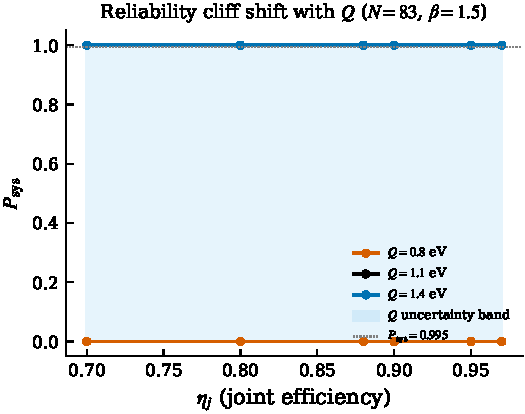
\includegraphics[width=\linewidth]{figures/fig_Q_reliability_envelope.pdf}
    \caption{$P_{\mathrm{sys}}$ vs.\ $\eta_j$ showing $Q$ uncertainty band ($N{=}83$, $\beta{=}1.5$).}
    \label{fig:q-envelope}
\end{figure}

\begin{figure}[h]
    \centering
    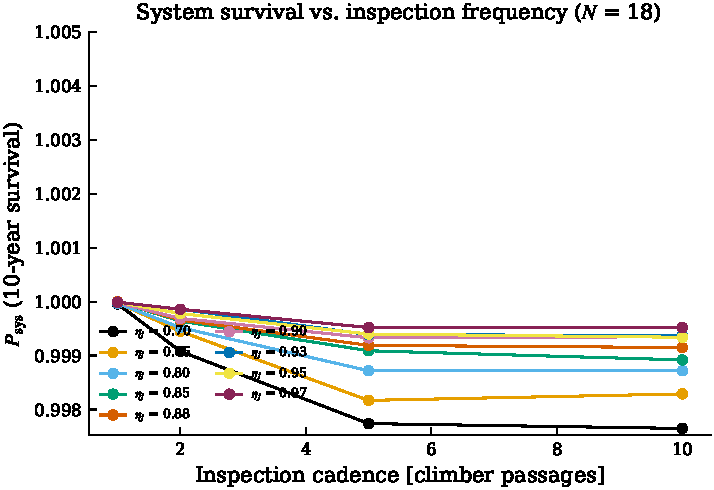
\includegraphics[width=0.85\linewidth]{figures/fig_inspection_cadence.pdf}
    \caption{System survival vs.\ inspection frequency.}
    \label{fig:inspection-cadence}
\end{figure}

\begin{figure}[h]
    \centering
    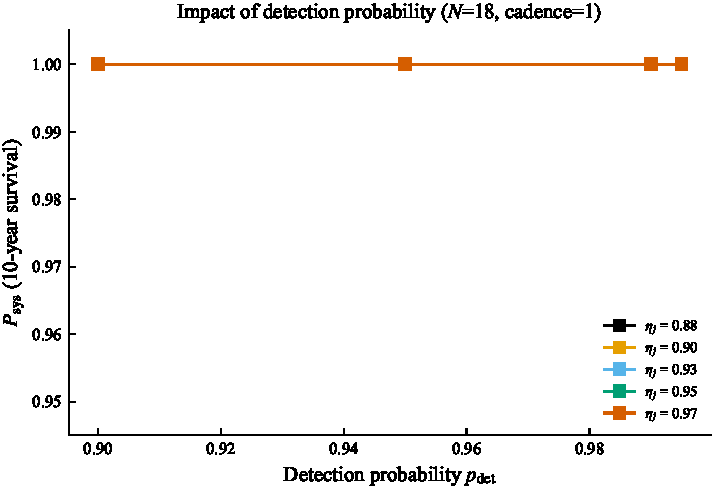
\includegraphics[width=0.85\linewidth]{figures/fig_p_detection_impact.pdf}
    \caption{$P_{\mathrm{sys}}$ vs.\ detection probability.}
    \label{fig:p-detection}
\end{figure}

\begin{figure}[h]
    \centering
    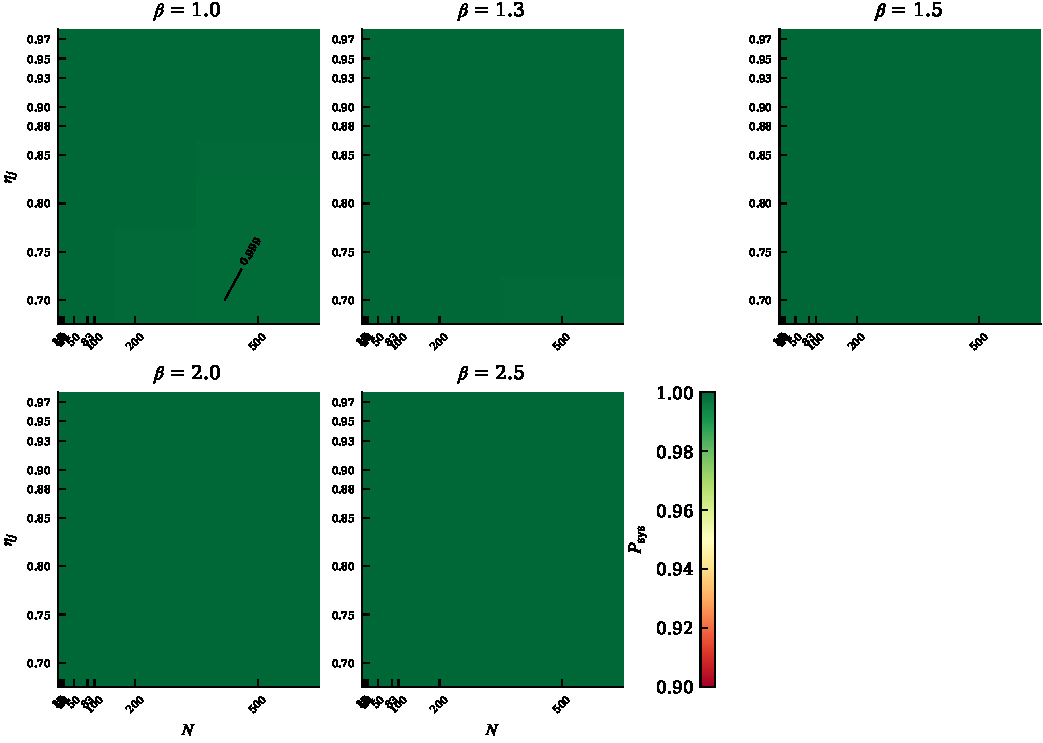
\includegraphics[width=\linewidth]{figures/fig_reliability_surface_by_beta.pdf}
    \caption{$P_{\mathrm{sys}}(N, \eta_j)$ heatmaps at each $\beta$ (5 panels).}
    \label{fig:reliability-by-beta}
\end{figure}

\begin{figure}[h]
    \centering
    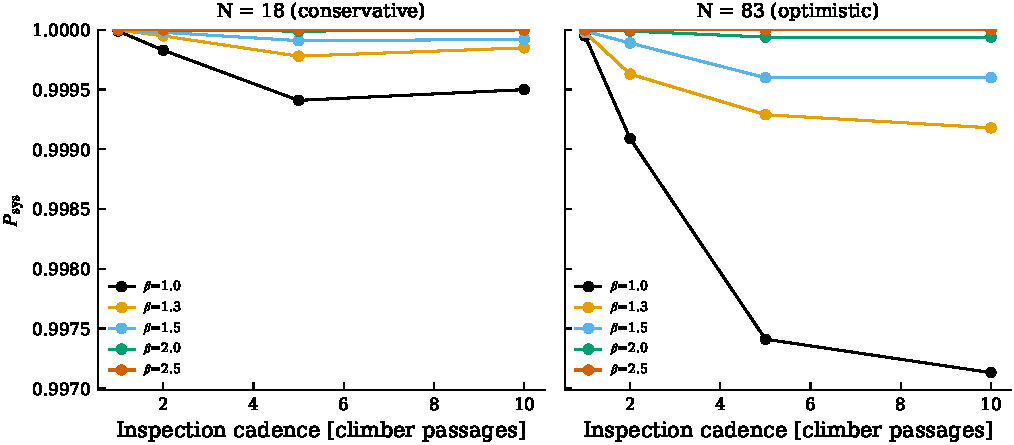
\includegraphics[width=0.85\linewidth]{figures/fig_cadence_sensitivity_by_beta.pdf}
    \caption{Inspection cadence sensitivity under wear-out.}
    \label{fig:cadence-by-beta}
\end{figure}

\begin{figure}[h]
    \centering
    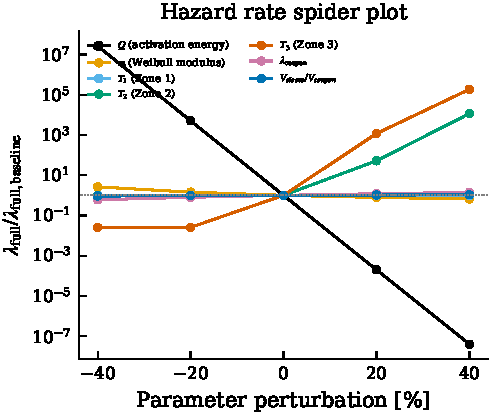
\includegraphics[width=0.75\linewidth]{figures/fig_hazard_spider.pdf}
    \caption{Hazard rate spider plot.}
    \label{fig:spider}
\end{figure}

\begin{figure}[h]
    \centering
    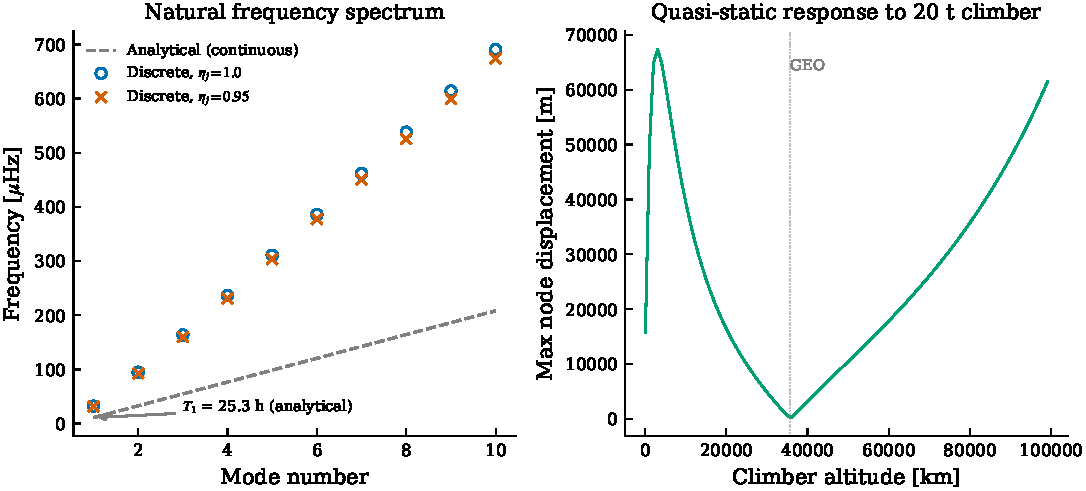
\includegraphics[width=0.85\linewidth]{figures/fig_modal_comparison.pdf}
    \caption{1D modal frequency spectrum and quasi-static forced response.}
    \label{fig:modal-1d}
\end{figure}

\begin{figure}[h]
    \centering
    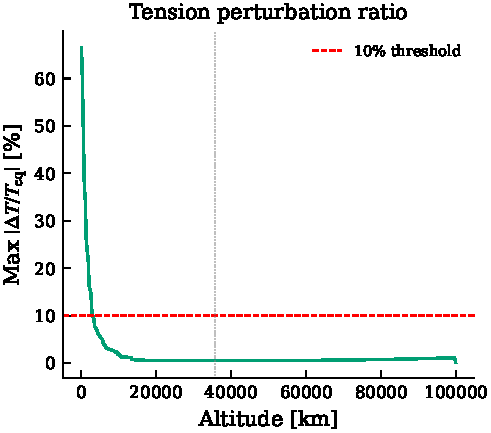
\includegraphics[width=0.85\linewidth]{figures/fig_tension_perturbation.pdf}
    \caption{Tension perturbation ratio $\Delta T / T_{\mathrm{eq}}$ vs.\ altitude.}
    \label{fig:tension-perturbation}
\end{figure}

\begin{figure}[h]
    \centering
    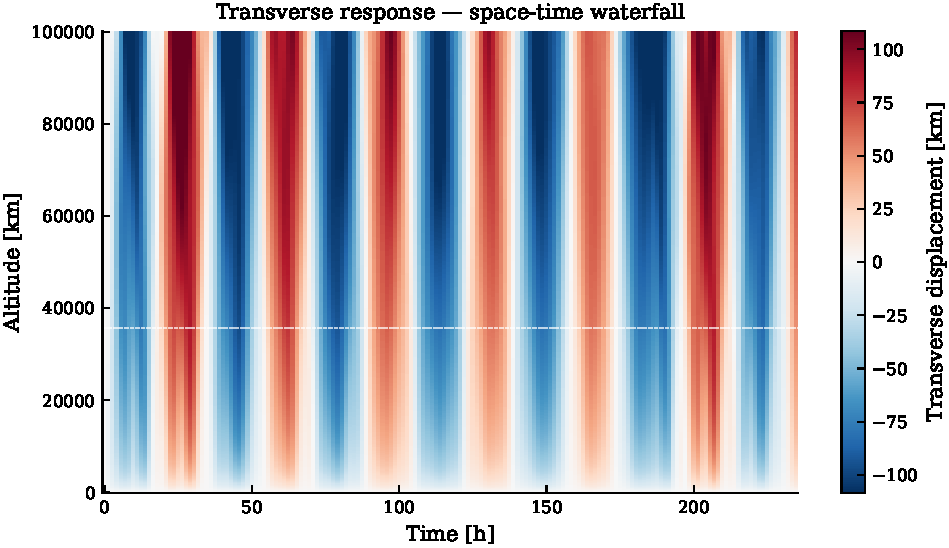
\includegraphics[width=\linewidth]{figures/fig_waterfall_vrt.pdf}
    \caption{Transverse response space-time waterfall $v(r, t)$.}
    \label{fig:waterfall}
\end{figure}

\begin{figure}[h]
    \centering
    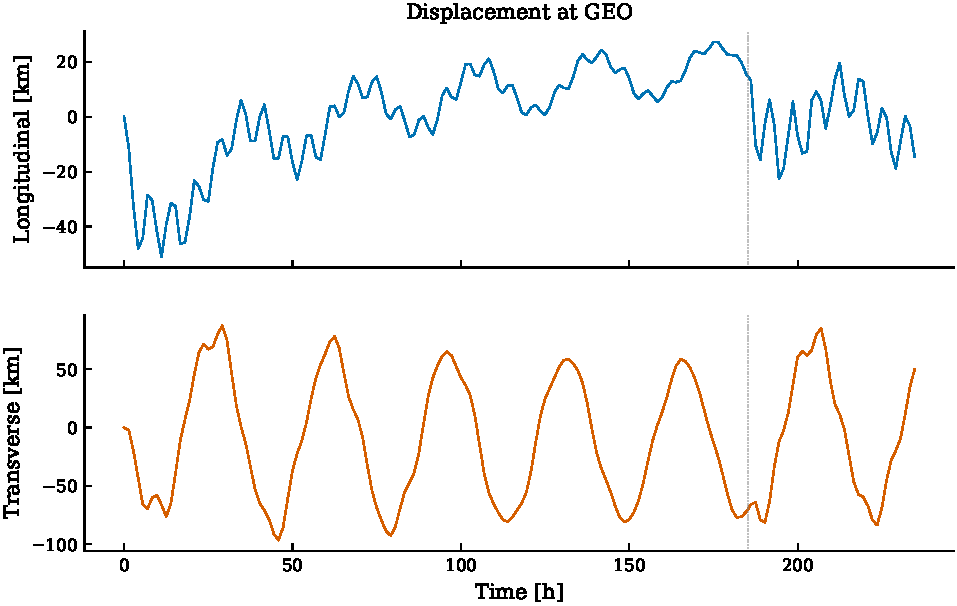
\includegraphics[width=0.85\linewidth]{figures/fig_geo_time_history.pdf}
    \caption{Displacement time history at GEO ($u$ and $v$).}
    \label{fig:geo-time-history}
\end{figure}

\begin{figure}[h]
    \centering
    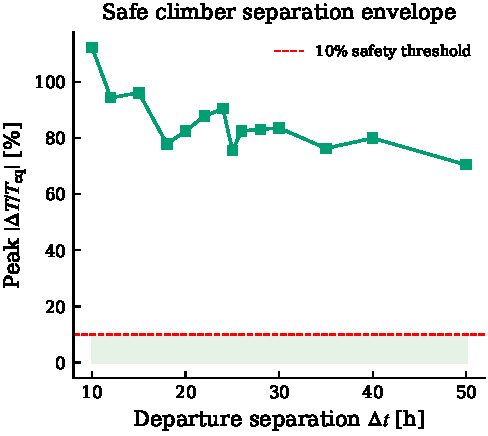
\includegraphics[width=0.85\linewidth]{figures/fig_safe_separation.pdf}
    \caption{Tension perturbation ratio vs.\ departure separation.}
    \label{fig:safe-separation}
\end{figure}

\begin{figure}[h]
    \centering
    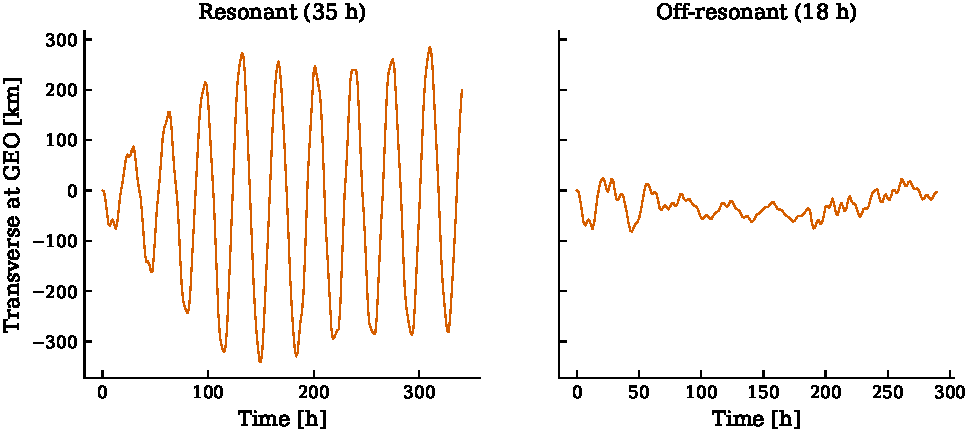
\includegraphics[width=0.85\linewidth]{figures/fig_resonant_vs_offresonant.pdf}
    \caption{GEO transverse displacement: resonant vs.\ off-resonant.}
    \label{fig:resonant-vs-off}
\end{figure}

\begin{figure}[h]
    \centering
    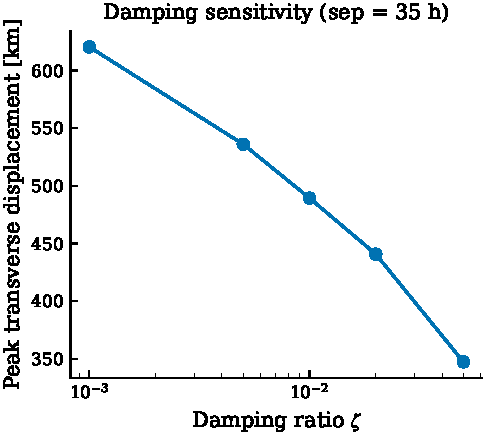
\includegraphics[width=0.75\linewidth]{figures/fig_damping_sensitivity.pdf}
    \caption{Peak transverse displacement vs.\ damping ratio $\zeta$.}
    \label{fig:damping}
\end{figure}

\begin{figure}[h]
    \centering
    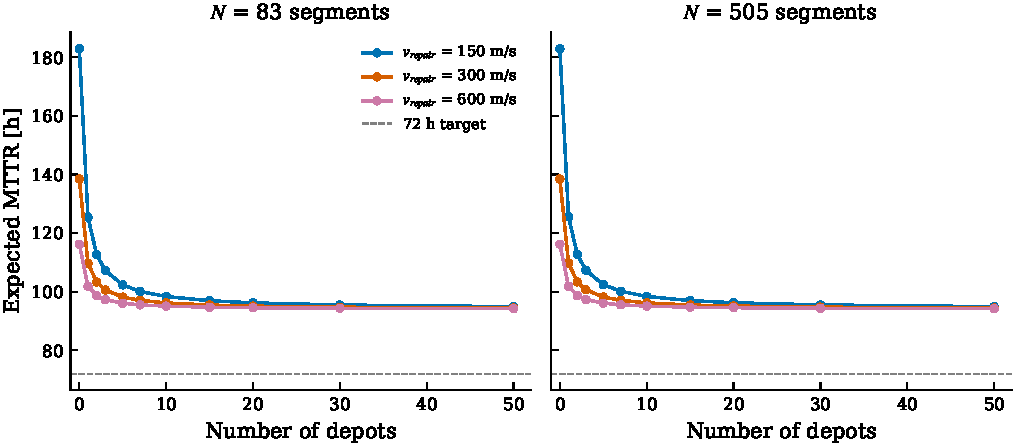
\includegraphics[width=0.85\linewidth]{figures/fig_mttr_vs_depots.pdf}
    \caption{Expected MTTR vs.\ depot count at $v_{\mathrm{repair}} = \{150, 300, 600\}$~m/s.}
    \label{fig:mttr-vs-depots}
\end{figure}

\begin{figure}[h]
    \centering
    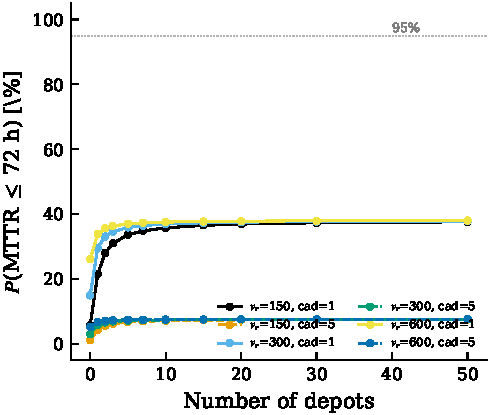
\includegraphics[width=0.75\linewidth]{figures/fig_72h_achievability.pdf}
    \caption{$P(\mathrm{MTTR} \leq \SI{72}{h})$ vs.\ depot count.}
    \label{fig:72h}
\end{figure}

\begin{figure}[h]
    \centering
    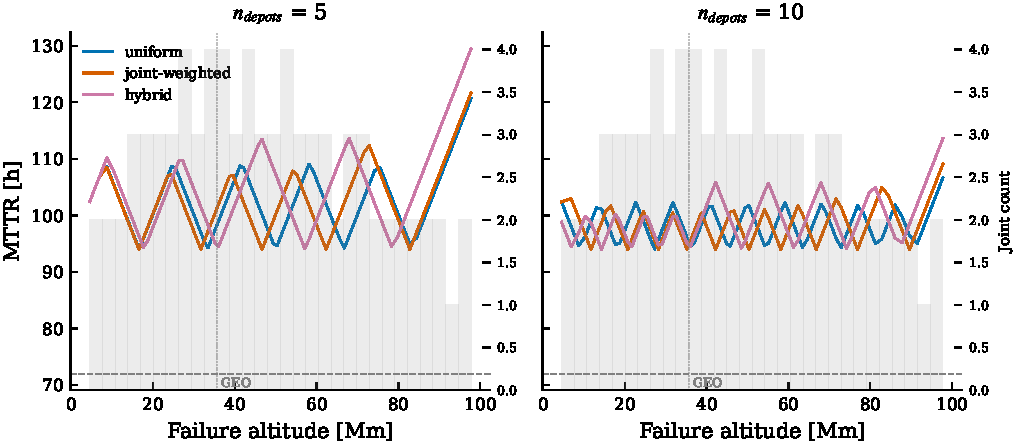
\includegraphics[width=0.85\linewidth]{figures/fig_depot_placement_comparison.pdf}
    \caption{MTTR vs.\ failure altitude for three placement strategies.}
    \label{fig:depot-placement}
\end{figure}

\begin{figure}[h]
    \centering
    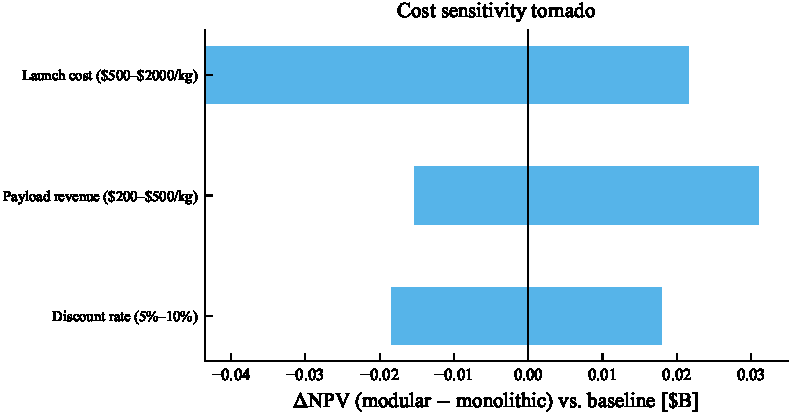
\includegraphics[width=0.85\linewidth]{figures/fig_cost_tornado.pdf}
    \caption{Cost sensitivity tornado diagram.}
    \label{fig:cost-tornado}
\end{figure}

\begin{figure}[h]
    \centering
    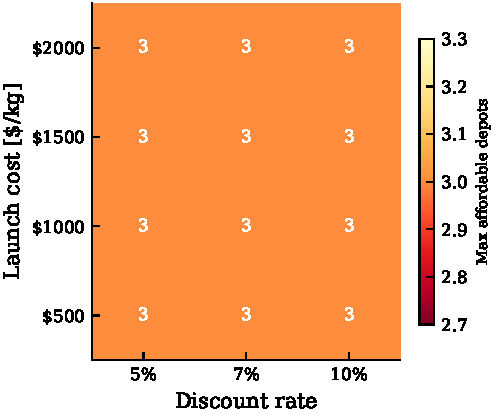
\includegraphics[width=0.75\linewidth]{figures/fig_depot_breakeven.pdf}
    \caption{Maximum affordable depots vs.\ scenario parameters.}
    \label{fig:depot-breakeven}
\end{figure}

\begin{figure}[h]
    \centering
    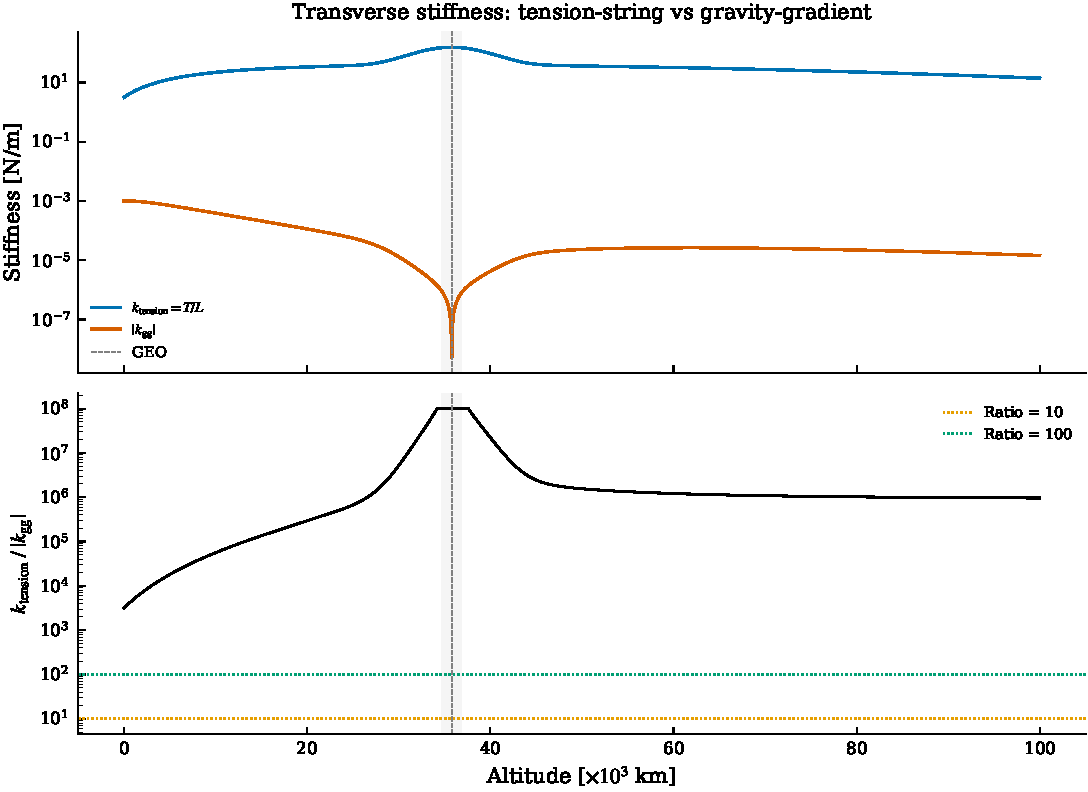
\includegraphics[width=0.85\linewidth]{figures/fig_stiffness_ratio.pdf}
    \caption{Tension vs.\ gravity-gradient stiffness comparison (2-panel).}
    \label{fig:stiffness-ratio}
\end{figure}

\begin{figure}[h]
    \centering
    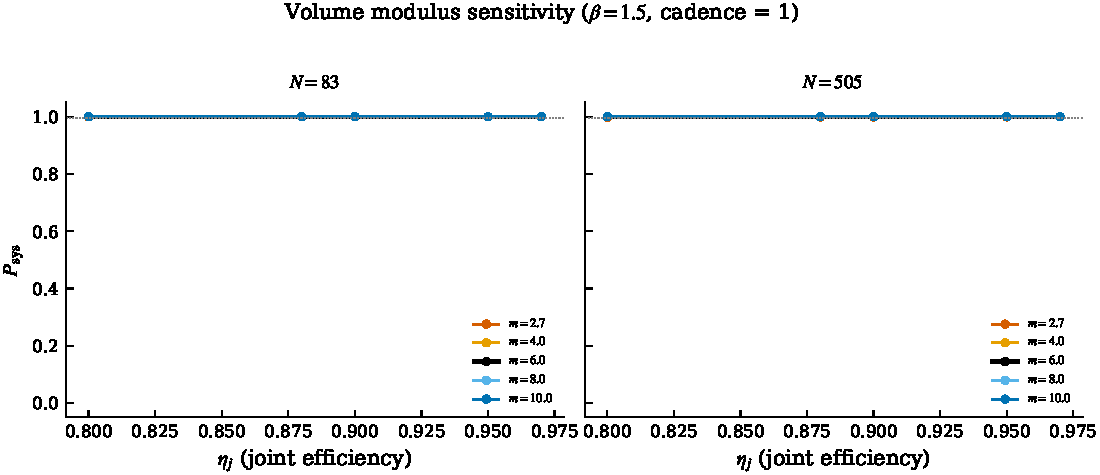
\includegraphics[width=0.85\linewidth]{figures/fig_volume_modulus_psys.pdf}
    \caption{$P_{\mathrm{sys}}$ vs.\ $\eta_j$ at Weibull volume moduli $m \in \{2.7, 4, 6, 8, 10\}$.}
    \label{fig:volume-modulus}
\end{figure}

%----------------------------------------------------------------------
% CRediT Author Statement
%----------------------------------------------------------------------

\section*{Author Contributions}

\textbf{K.\ Egan:} Conceptualization, Methodology, Software, Formal Analysis, Writing---Original Draft, Visualization.

\end{document}
